\documentclass[]{elsarticle} %review=doublespace preprint=single 5p=2 column
%%% Begin My package additions %%%%%%%%%%%%%%%%%%%

\usepackage[hyphens]{url}


\usepackage{lineno} % add
  \linenumbers % turns line numbering on

\usepackage{graphicx}
%%%%%%%%%%%%%%%% end my additions to header

\usepackage[T1]{fontenc}
\usepackage{lmodern}
\usepackage{amssymb,amsmath}
\usepackage{ifxetex,ifluatex}
\usepackage{fixltx2e} % provides \textsubscript
% use upquote if available, for straight quotes in verbatim environments
\IfFileExists{upquote.sty}{\usepackage{upquote}}{}
\ifnum 0\ifxetex 1\fi\ifluatex 1\fi=0 % if pdftex
  \usepackage[utf8]{inputenc}
\else % if luatex or xelatex
  \usepackage{fontspec}
  \ifxetex
    \usepackage{xltxtra,xunicode}
  \fi
  \defaultfontfeatures{Mapping=tex-text,Scale=MatchLowercase}
  \newcommand{\euro}{€}
\fi
% use microtype if available
\IfFileExists{microtype.sty}{\usepackage{microtype}}{}
\usepackage[]{natbib}
\bibliographystyle{plainnat}

\ifxetex
  \usepackage[setpagesize=false, % page size defined by xetex
              unicode=false, % unicode breaks when used with xetex
              xetex]{hyperref}
\else
  \usepackage[unicode=true]{hyperref}
\fi
\hypersetup{breaklinks=true,
            bookmarks=true,
            pdfauthor={},
            pdftitle={Supplementary Information part 2: Testing the improved data sets},
            colorlinks=false,
            urlcolor=blue,
            linkcolor=magenta,
            pdfborder={0 0 0}}

\setcounter{secnumdepth}{5}
% Pandoc toggle for numbering sections (defaults to be off)

% Pandoc syntax highlighting
\usepackage{color}
\usepackage{fancyvrb}
\newcommand{\VerbBar}{|}
\newcommand{\VERB}{\Verb[commandchars=\\\{\}]}
\DefineVerbatimEnvironment{Highlighting}{Verbatim}{commandchars=\\\{\}}
% Add ',fontsize=\small' for more characters per line
\usepackage{framed}
\definecolor{shadecolor}{RGB}{248,248,248}
\newenvironment{Shaded}{\begin{snugshade}}{\end{snugshade}}
\newcommand{\AlertTok}[1]{\textcolor[rgb]{0.94,0.16,0.16}{#1}}
\newcommand{\AnnotationTok}[1]{\textcolor[rgb]{0.56,0.35,0.01}{\textbf{\textit{#1}}}}
\newcommand{\AttributeTok}[1]{\textcolor[rgb]{0.77,0.63,0.00}{#1}}
\newcommand{\BaseNTok}[1]{\textcolor[rgb]{0.00,0.00,0.81}{#1}}
\newcommand{\BuiltInTok}[1]{#1}
\newcommand{\CharTok}[1]{\textcolor[rgb]{0.31,0.60,0.02}{#1}}
\newcommand{\CommentTok}[1]{\textcolor[rgb]{0.56,0.35,0.01}{\textit{#1}}}
\newcommand{\CommentVarTok}[1]{\textcolor[rgb]{0.56,0.35,0.01}{\textbf{\textit{#1}}}}
\newcommand{\ConstantTok}[1]{\textcolor[rgb]{0.00,0.00,0.00}{#1}}
\newcommand{\ControlFlowTok}[1]{\textcolor[rgb]{0.13,0.29,0.53}{\textbf{#1}}}
\newcommand{\DataTypeTok}[1]{\textcolor[rgb]{0.13,0.29,0.53}{#1}}
\newcommand{\DecValTok}[1]{\textcolor[rgb]{0.00,0.00,0.81}{#1}}
\newcommand{\DocumentationTok}[1]{\textcolor[rgb]{0.56,0.35,0.01}{\textbf{\textit{#1}}}}
\newcommand{\ErrorTok}[1]{\textcolor[rgb]{0.64,0.00,0.00}{\textbf{#1}}}
\newcommand{\ExtensionTok}[1]{#1}
\newcommand{\FloatTok}[1]{\textcolor[rgb]{0.00,0.00,0.81}{#1}}
\newcommand{\FunctionTok}[1]{\textcolor[rgb]{0.00,0.00,0.00}{#1}}
\newcommand{\ImportTok}[1]{#1}
\newcommand{\InformationTok}[1]{\textcolor[rgb]{0.56,0.35,0.01}{\textbf{\textit{#1}}}}
\newcommand{\KeywordTok}[1]{\textcolor[rgb]{0.13,0.29,0.53}{\textbf{#1}}}
\newcommand{\NormalTok}[1]{#1}
\newcommand{\OperatorTok}[1]{\textcolor[rgb]{0.81,0.36,0.00}{\textbf{#1}}}
\newcommand{\OtherTok}[1]{\textcolor[rgb]{0.56,0.35,0.01}{#1}}
\newcommand{\PreprocessorTok}[1]{\textcolor[rgb]{0.56,0.35,0.01}{\textit{#1}}}
\newcommand{\RegionMarkerTok}[1]{#1}
\newcommand{\SpecialCharTok}[1]{\textcolor[rgb]{0.00,0.00,0.00}{#1}}
\newcommand{\SpecialStringTok}[1]{\textcolor[rgb]{0.31,0.60,0.02}{#1}}
\newcommand{\StringTok}[1]{\textcolor[rgb]{0.31,0.60,0.02}{#1}}
\newcommand{\VariableTok}[1]{\textcolor[rgb]{0.00,0.00,0.00}{#1}}
\newcommand{\VerbatimStringTok}[1]{\textcolor[rgb]{0.31,0.60,0.02}{#1}}
\newcommand{\WarningTok}[1]{\textcolor[rgb]{0.56,0.35,0.01}{\textbf{\textit{#1}}}}

% tightlist command for lists without linebreak
\providecommand{\tightlist}{%
  \setlength{\itemsep}{0pt}\setlength{\parskip}{0pt}}

% From pandoc table feature
\usepackage{longtable,booktabs,array}
\usepackage{calc} % for calculating minipage widths
% Correct order of tables after \paragraph or \subparagraph
\usepackage{etoolbox}
\makeatletter
\patchcmd\longtable{\par}{\if@noskipsec\mbox{}\fi\par}{}{}
\makeatother
% Allow footnotes in longtable head/foot
\IfFileExists{footnotehyper.sty}{\usepackage{footnotehyper}}{\usepackage{footnote}}
\makesavenoteenv{longtable}


\usepackage{setspace}
\usepackage{color}
\newcommand{\beginsupplement}{  \setcounter{table}{0} \renewcommand{\thetable}{S\arabic{table}} \setcounter{figure}{0} \renewcommand{\thefigure}{S\arabic{figure}}}



\begin{document}


\begin{frontmatter}

  \title{Supplementary Information part 2: Testing the improved data sets}
    \author[]{R. Willem Vervoort%
  %
  \fnref{1}}
   \ead{willem.vervoort@sydney.edu.au} 
    \author[]{Eliana Nervi}
   \ead{eliananervif@gmail.com} 
    \author[]{Jimena Alonso}
   \ead{jalonso@fing.edu.uy} 
      \cortext[cor1]{Corresponding author}
    \fntext[1]{Corresponding Author}
  
  \begin{abstract}
  This supplementary material file compares whether the inclusion of additional catchments generates fundamentally different results as the original (but improved) data. Single variable regressions on the smaller (original) dataset are compared with the extended data set.
  \end{abstract}
  
 \end{frontmatter}

\setcounter{table}{0} \renewcommand{\thetable}{S\arabic{table}} \setcounter{figure}{0} \renewcommand{\thefigure}{S\arabic{figure}}

\hypertarget{introduction}{%
\section{Introduction}\label{introduction}}

This supplementary material is related to `Generalizing the impact of forest cover on streamflow from experimental data: it is not that simple. Vervoort et al.'

In this document we tested whether the fundamental conclusions in the single variable regressions with the improved data base differed from the original conclusions in \citet{zhang2017}. This is to check how much influence the changes to the data set and the additional data might have changed the original conclusions.

\hypertarget{methods}{%
\section{Methods}\label{methods}}

First we will read in the data

We will combine the different tables, but will keep an indicator to see where the data are from.

\begin{Shaded}
\begin{Highlighting}[]
\NormalTok{Zhang\_small}\SpecialCharTok{$}\NormalTok{From }\OtherTok{\textless{}{-}} \FunctionTok{as.numeric}\NormalTok{(Zhang\_small}\SpecialCharTok{$}\NormalTok{From)}
\NormalTok{Zhang\_small}\SpecialCharTok{$}\NormalTok{To }\OtherTok{\textless{}{-}} \FunctionTok{as.numeric}\NormalTok{(Zhang\_small}\SpecialCharTok{$}\NormalTok{To)}
\NormalTok{Zhang\_all }\OtherTok{\textless{}{-}} \FunctionTok{bind\_rows}\NormalTok{(Zhang\_large,Zhang\_small) }\SpecialCharTok{\%\textgreater{}\%}
  \FunctionTok{mutate}\NormalTok{(}\AttributeTok{dataset =} \StringTok{"original Zhang et al data"}\NormalTok{)}
\NormalTok{new\_data }\OtherTok{\textless{}{-}}\NormalTok{ new\_data }\SpecialCharTok{\%\textgreater{}\%}
  \FunctionTok{mutate}\NormalTok{(}\AttributeTok{dataset =} \StringTok{"new data"}\NormalTok{)}
\NormalTok{All\_data }\OtherTok{\textless{}{-}} \FunctionTok{bind\_rows}\NormalTok{(Zhang\_all, new\_data)}
\end{Highlighting}
\end{Shaded}

\hypertarget{implementing-the-changes-to-the-overall-data}{%
\section{Implementing the changes to the overall data}\label{implementing-the-changes-to-the-overall-data}}

The following code implements the changes described in the Supplementary data part 1. However, many of the changes were implemented manually into the data set. These are simply the remaining changes not implemented manually.

\begin{enumerate}
\def\labelenumi{\arabic{enumi}.}
\tightlist
\item
  removing the duplicates.
\end{enumerate}

\begin{Shaded}
\begin{Highlighting}[]
\NormalTok{All\_data }\OtherTok{\textless{}{-}}\NormalTok{ All\_data }\SpecialCharTok{\%\textgreater{}\%}
  \FunctionTok{mutate}\NormalTok{(}\StringTok{\textasciigrave{}}\AttributeTok{Possible duplicate}\StringTok{\textasciigrave{}} \OtherTok{=} 
           \FunctionTok{ifelse}\NormalTok{(}\FunctionTok{is.na}\NormalTok{(}\StringTok{\textasciigrave{}}\AttributeTok{Possible duplicate}\StringTok{\textasciigrave{}}\NormalTok{)}\SpecialCharTok{==}\NormalTok{T,}\DecValTok{0}\NormalTok{,}\StringTok{\textasciigrave{}}\AttributeTok{Possible duplicate}\StringTok{\textasciigrave{}}\NormalTok{),}
         \StringTok{\textasciigrave{}}\AttributeTok{Possible duplicate}\StringTok{\textasciigrave{}} \OtherTok{=} \FunctionTok{as.numeric}\NormalTok{(}\StringTok{\textasciigrave{}}\AttributeTok{Possible duplicate}\StringTok{\textasciigrave{}}\NormalTok{)) }\SpecialCharTok{\%\textgreater{}\%}
  \FunctionTok{filter}\NormalTok{(}\StringTok{\textasciigrave{}}\AttributeTok{Possible duplicate}\StringTok{\textasciigrave{}} \SpecialCharTok{!=} \DecValTok{1}\NormalTok{)}
\end{Highlighting}
\end{Shaded}

\begin{enumerate}
\def\labelenumi{\arabic{enumi}.}
\setcounter{enumi}{1}
\tightlist
\item
  calculating the dryness
\end{enumerate}

\begin{Shaded}
\begin{Highlighting}[]
\CommentTok{\# calculate dryness index}
\NormalTok{All\_data }\OtherTok{\textless{}{-}}\NormalTok{ All\_data }\SpecialCharTok{\%\textgreater{}\%}
  \FunctionTok{mutate}\NormalTok{(}\AttributeTok{Dryness =}\NormalTok{ E0}\SpecialCharTok{/}\NormalTok{Pa\_mm)}
\end{Highlighting}
\end{Shaded}

\begin{enumerate}
\def\labelenumi{\arabic{enumi}.}
\setcounter{enumi}{2}
\tightlist
\item
  remove watershed 1 (the Amazon) from the analysis
\end{enumerate}

\begin{Shaded}
\begin{Highlighting}[]
\NormalTok{All\_data }\OtherTok{\textless{}{-}}\NormalTok{ All\_data }\SpecialCharTok{\%\textgreater{}\%}
  \FunctionTok{filter}\NormalTok{(}\StringTok{\textasciigrave{}}\AttributeTok{Watershed \#}\StringTok{\textasciigrave{}} \SpecialCharTok{!=} \DecValTok{1}\NormalTok{)}
\end{Highlighting}
\end{Shaded}

\begin{enumerate}
\def\labelenumi{\arabic{enumi}.}
\setcounter{enumi}{3}
\tightlist
\item
  remove data set 188 and 254 Kamakia and Sambret
\end{enumerate}

\begin{Shaded}
\begin{Highlighting}[]
\NormalTok{All\_data }\OtherTok{\textless{}{-}}\NormalTok{ All\_data }\SpecialCharTok{\%\textgreater{}\%}
  \FunctionTok{filter}\NormalTok{(}\StringTok{\textasciigrave{}}\AttributeTok{Watershed \#}\StringTok{\textasciigrave{}} \SpecialCharTok{!=} \DecValTok{188}\NormalTok{) }\SpecialCharTok{\%\textgreater{}\%}
  \FunctionTok{filter}\NormalTok{(}\StringTok{\textasciigrave{}}\AttributeTok{Watershed \#}\StringTok{\textasciigrave{}} \SpecialCharTok{!=} \DecValTok{254}\NormalTok{)}
\end{Highlighting}
\end{Shaded}

\begin{enumerate}
\def\labelenumi{\arabic{enumi}.}
\setcounter{enumi}{4}
\tightlist
\item
  add a column that indicates forst loss of forest gain
\end{enumerate}

\begin{Shaded}
\begin{Highlighting}[]
\NormalTok{All\_data }\OtherTok{\textless{}{-}}\NormalTok{ All\_data }\SpecialCharTok{\%\textgreater{}\%}
  \FunctionTok{mutate}\NormalTok{(}\AttributeTok{forest\_sign =} \FunctionTok{ifelse}\NormalTok{(DeltaF\_perc }\SpecialCharTok{\textless{}} \DecValTok{0}\NormalTok{, }\StringTok{"Forest Cover Loss"}\NormalTok{, }\StringTok{"Forest Cover Gain"}\NormalTok{))}
\end{Highlighting}
\end{Shaded}

\hypertarget{approach-and-analyses}{%
\subsection{Approach and analyses}\label{approach-and-analyses}}

The approach is similar to \citet{zhang2017}. We run single variable regressions separating large (\textgreater{} 1000 km\textsuperscript{2}) and small catchments (\textless= 1000 km\textsuperscript{2}).

The paper by \citet{zhang2017} calculates the sensitivity of runoff as a function of runoff as:

\(\Delta Q_f = 100 \times \frac{\Delta Q_{f,mm}}{\bar{Q}}\)

This first equation is superfluous in this case as the data (as extracted from \citet{zhang2017}) is already defined in terms of \(\Delta Q_f\).

\(S_f = |\frac{\Delta Q_f}{\Delta F}|\)

\begin{Shaded}
\begin{Highlighting}[]
\NormalTok{All\_data }\OtherTok{\textless{}{-}}\NormalTok{ All\_data }\SpecialCharTok{\%\textgreater{}\%}
  \FunctionTok{filter}\NormalTok{(}\FunctionTok{is.na}\NormalTok{(DeltaF\_perc) }\SpecialCharTok{==}\NormalTok{ F) }\SpecialCharTok{\%\textgreater{}\%}
  \FunctionTok{mutate}\NormalTok{(}\AttributeTok{S\_f =} \FunctionTok{abs}\NormalTok{(DeltaQf\_perc}\SpecialCharTok{/}\NormalTok{DeltaF\_perc))}
\end{Highlighting}
\end{Shaded}

In sequence we analyse:

\begin{itemize}
\tightlist
\item
  the relationship between forest cover change and streamflow change for small and large catchments (i.e.~Figure 2 in \citet{zhang2017});\\
\item
  the relationship between catchment size and the sensitivity to runoff change (i.e.~Figure 3 in \citet{zhang2017}); and\\
\item
  the sensitivity to forest loss as a function of dryness (i.e.~Figure 4 in \citet{zhang2017}).
\end{itemize}

\hypertarget{results}{%
\section{Results}\label{results}}

\hypertarget{the-change-in-stream-flow-as-a-function-of-change-in-forest-cover}{%
\subsection{The change in stream flow as a function of change in forest cover}\label{the-change-in-stream-flow-as-a-function-of-change-in-forest-cover}}

Figure \ref{fig:Fig2Zhang} highlights that the overall relationship in the updated dataset is the same as in \citet{zhang2017}. This means that while the modifications have cleaned up the transcription errors in the data, they have not fundamentally changed the conclusions in the original paper.

The next figure (Figure \ref{fig:Fig2Zhangnew}) is the same analysis, but this includes the new data that we identified in papers. Again, this figure highlights that the new datasets have not fundamentally changed the relationships found in \citet{zhang2017}.

\begin{figure}
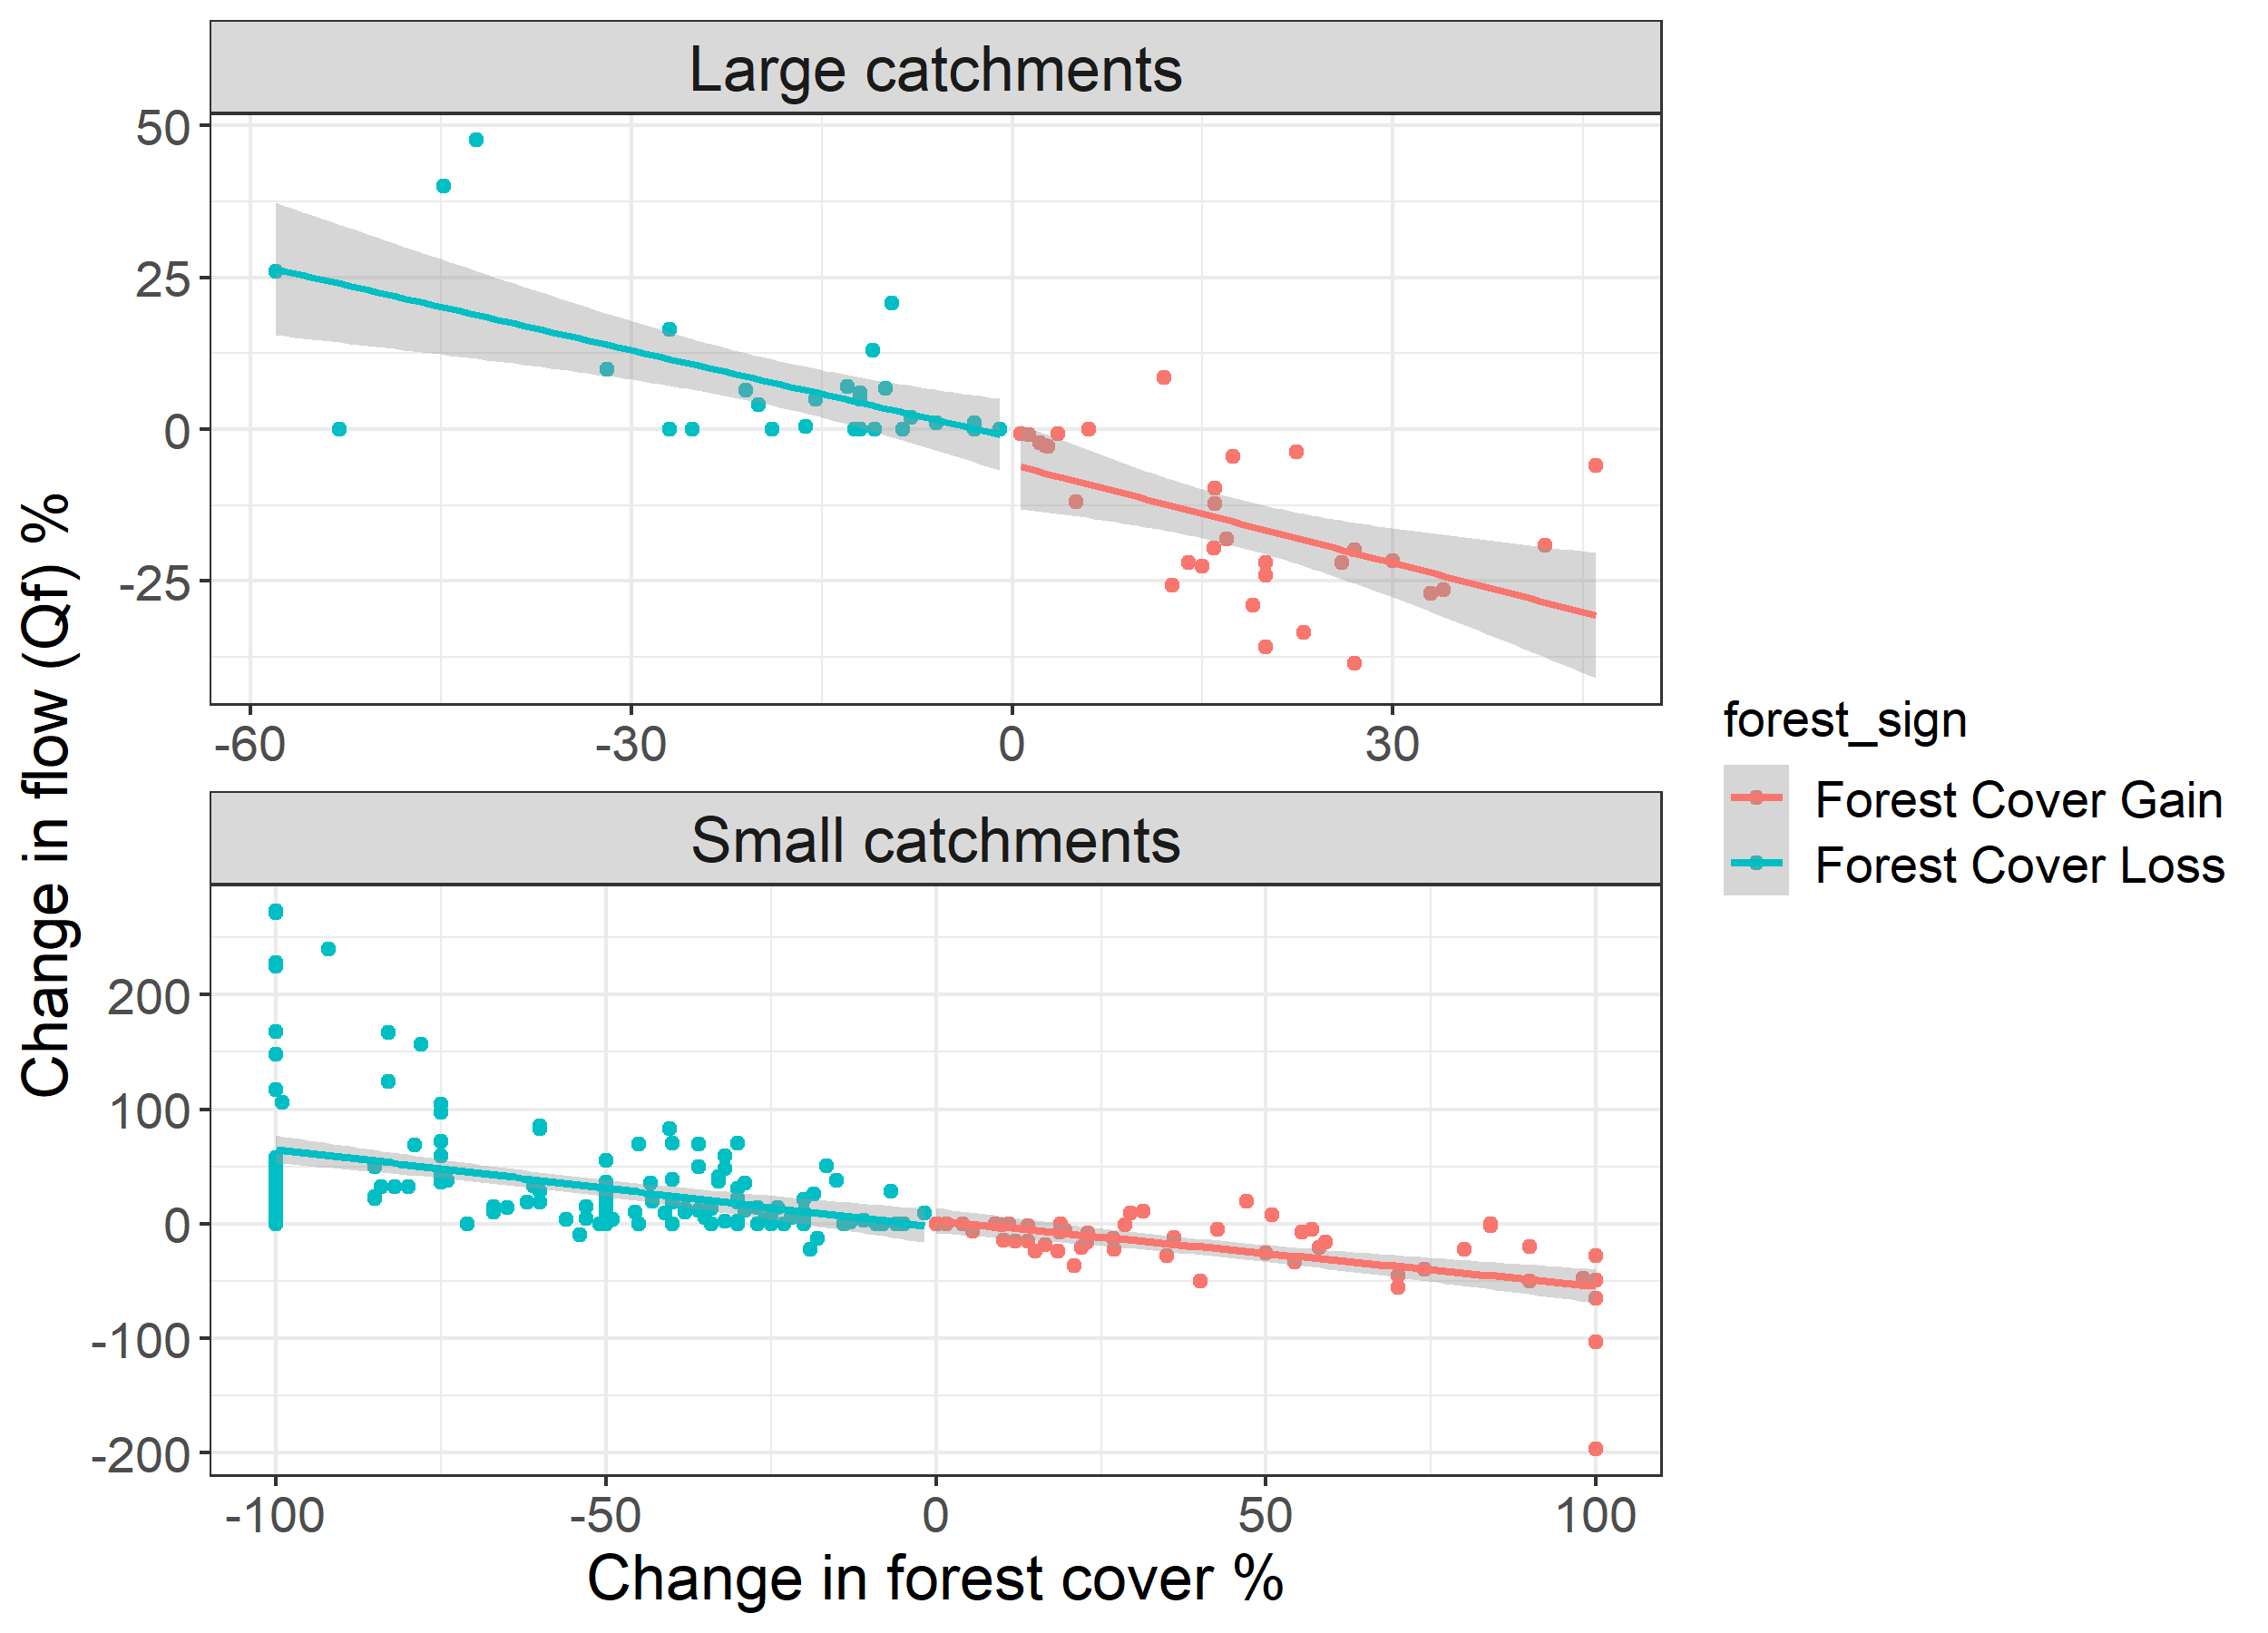
\includegraphics[width=0.9\linewidth]{Fig2Zhang} \caption{Changes in flow based on the catchments from the original data set}\label{fig:Fig2Zhang}
\end{figure}

\begin{figure}
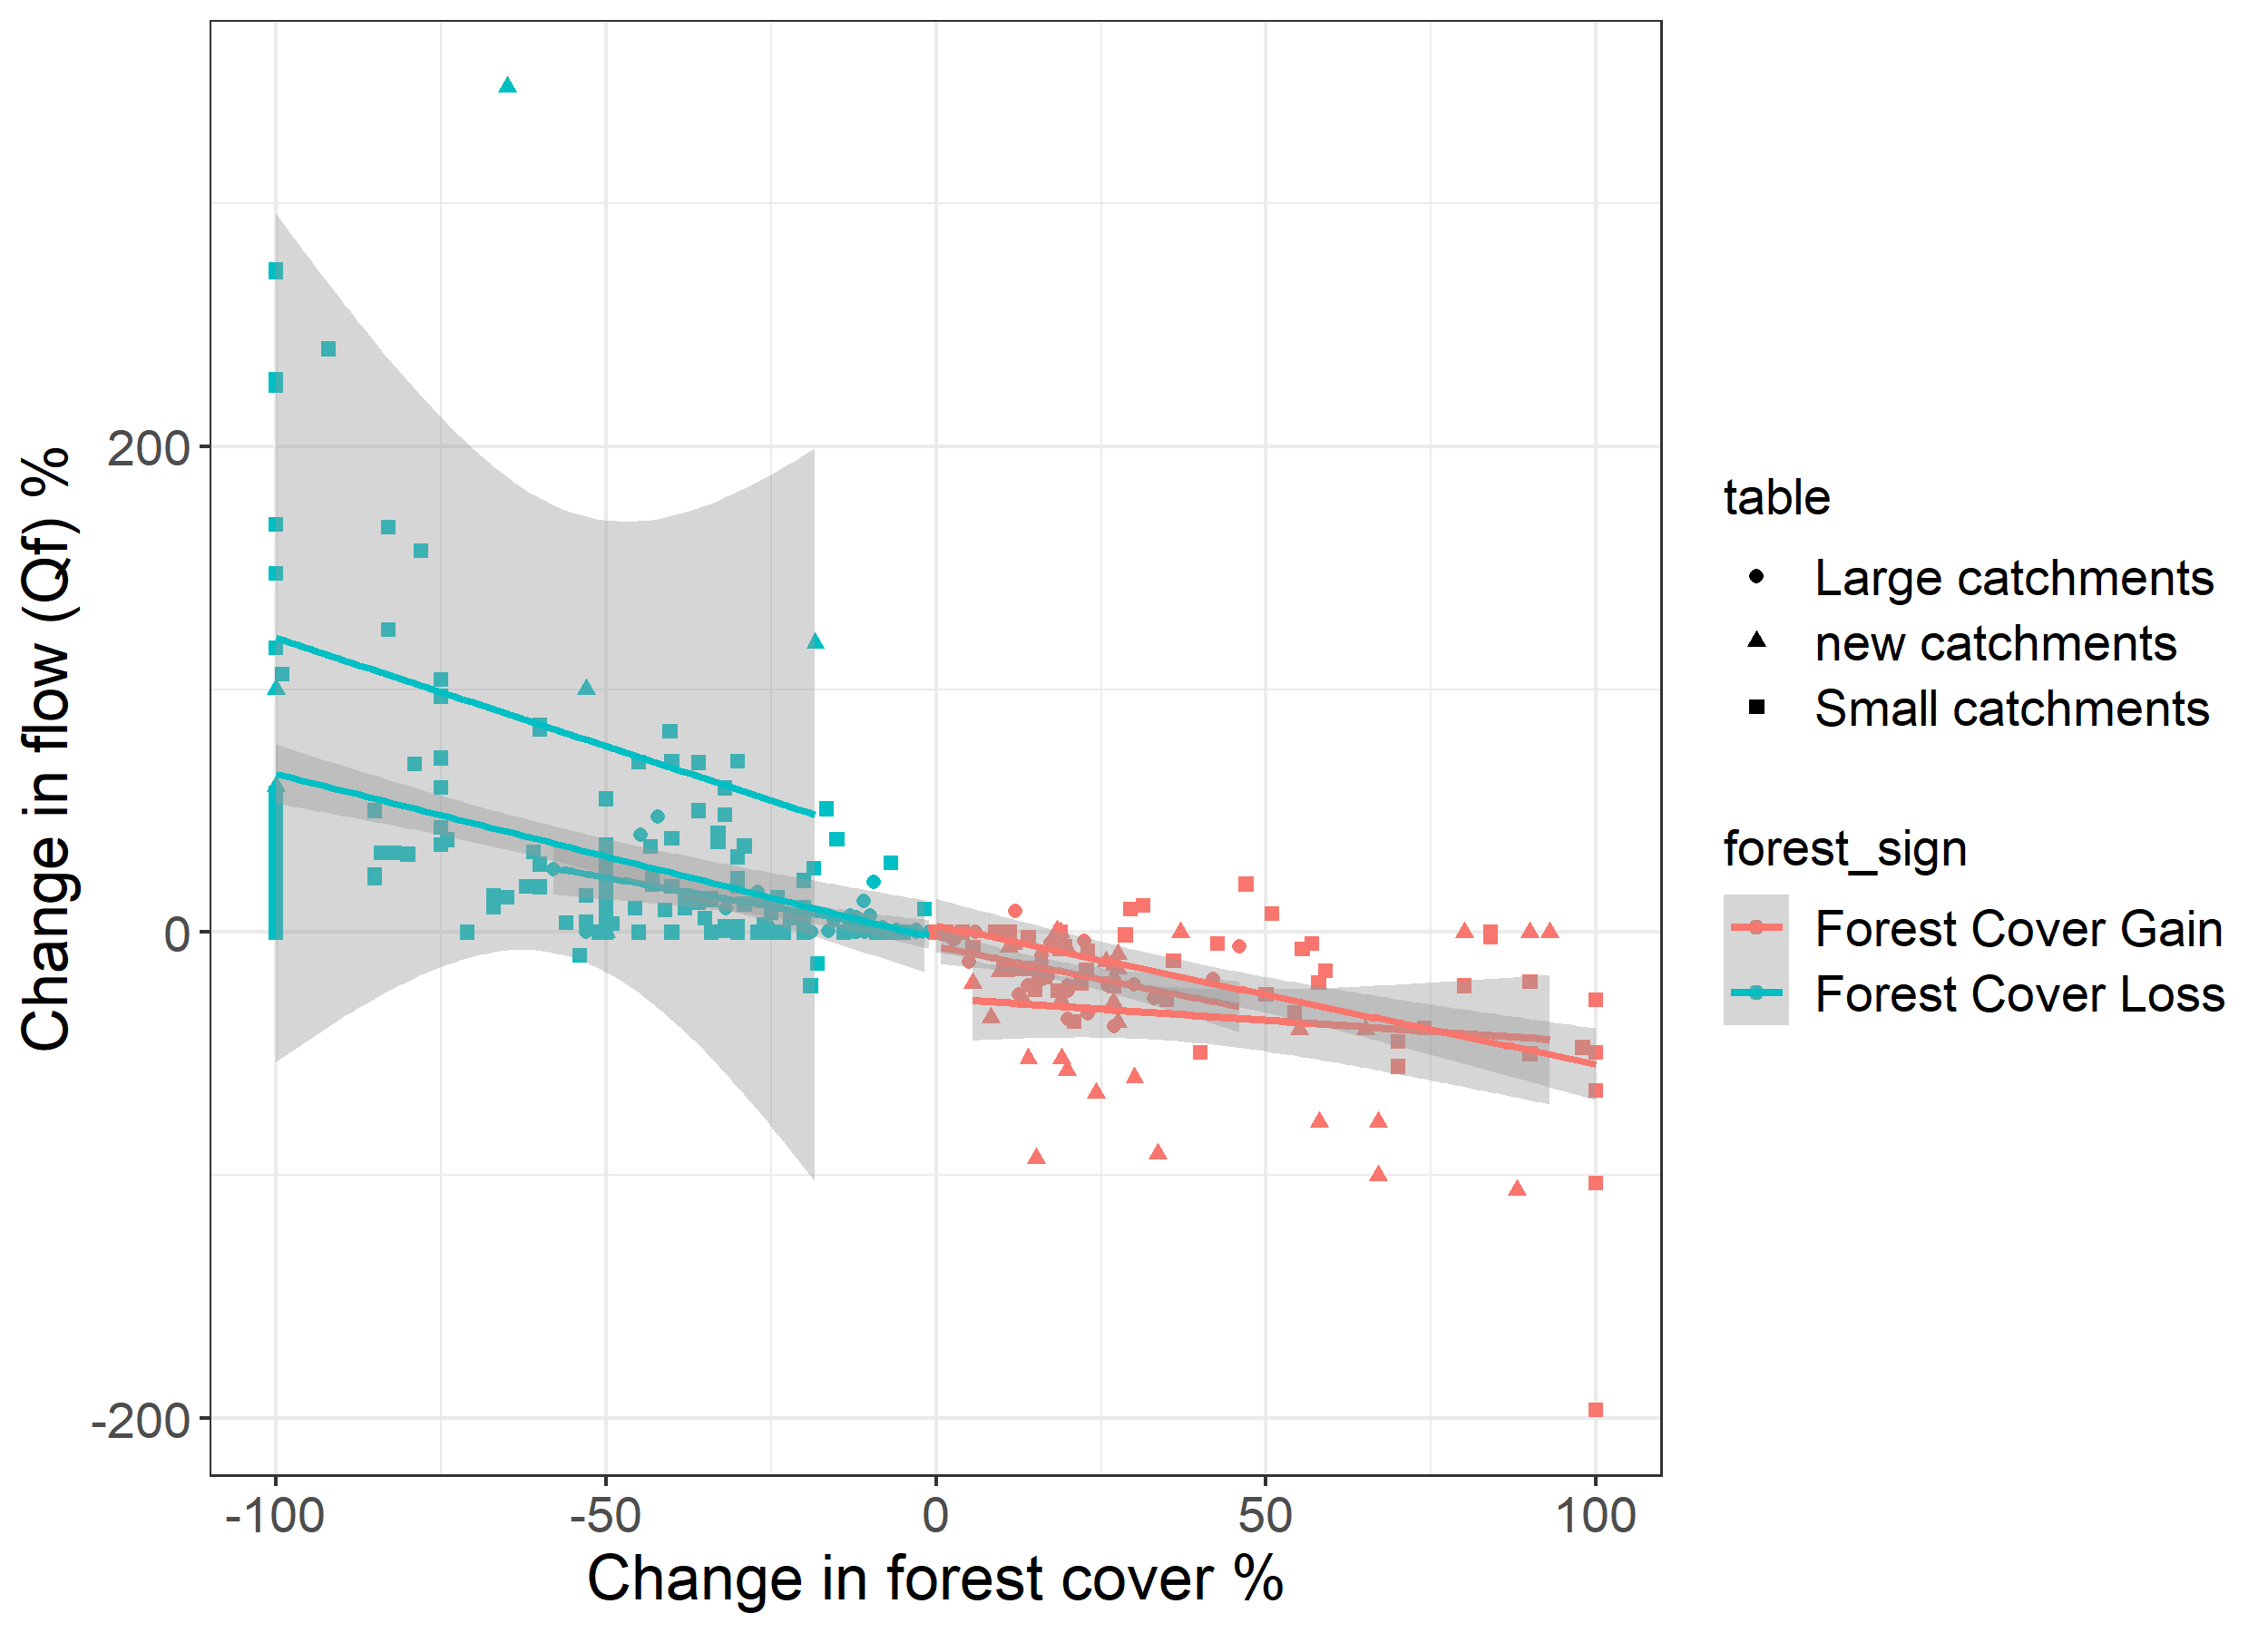
\includegraphics[width=0.9\linewidth]{Fig2Zhang_all} \caption{Changes in flow based on the catchments from the extended data set}\label{fig:Fig2Zhangnew}
\end{figure}

\hypertarget{the-relationship-between-the-area-of-the-catchment-and-the-sensitivity-of-streamflow-to-the-change-in-forest-cover.}{%
\subsection{The relationship between the area of the catchment and the sensitivity of streamflow to the change in forest cover.}\label{the-relationship-between-the-area-of-the-catchment-and-the-sensitivity-of-streamflow-to-the-change-in-forest-cover.}}

This analysis replicates Figure 3 in \citet{zhang2017}, which investigates for large and small catchments the sensitivity to runoff change from change in forest cover as a function of area. Note that in the original figure, the x-axis is on a log scale. In the original paper, the analysis is presented for all catchments as well as for large and small catchments. Here we only analyse the small and large catchments.

We can see from Figure \ref{fig:Fig3Zhang} that again the updated database for the original dataset results in little change in the relationships for both large and small catchments. However, when the additional new catchments are added to the database (Figure \ref{fig:Fig3Zhangnew}), the relationships clearly change. In particular, for small catchments gaining forest cover, the sensitivity appears positively correlated with the logarithm of the size of the catchments.

\begin{figure}
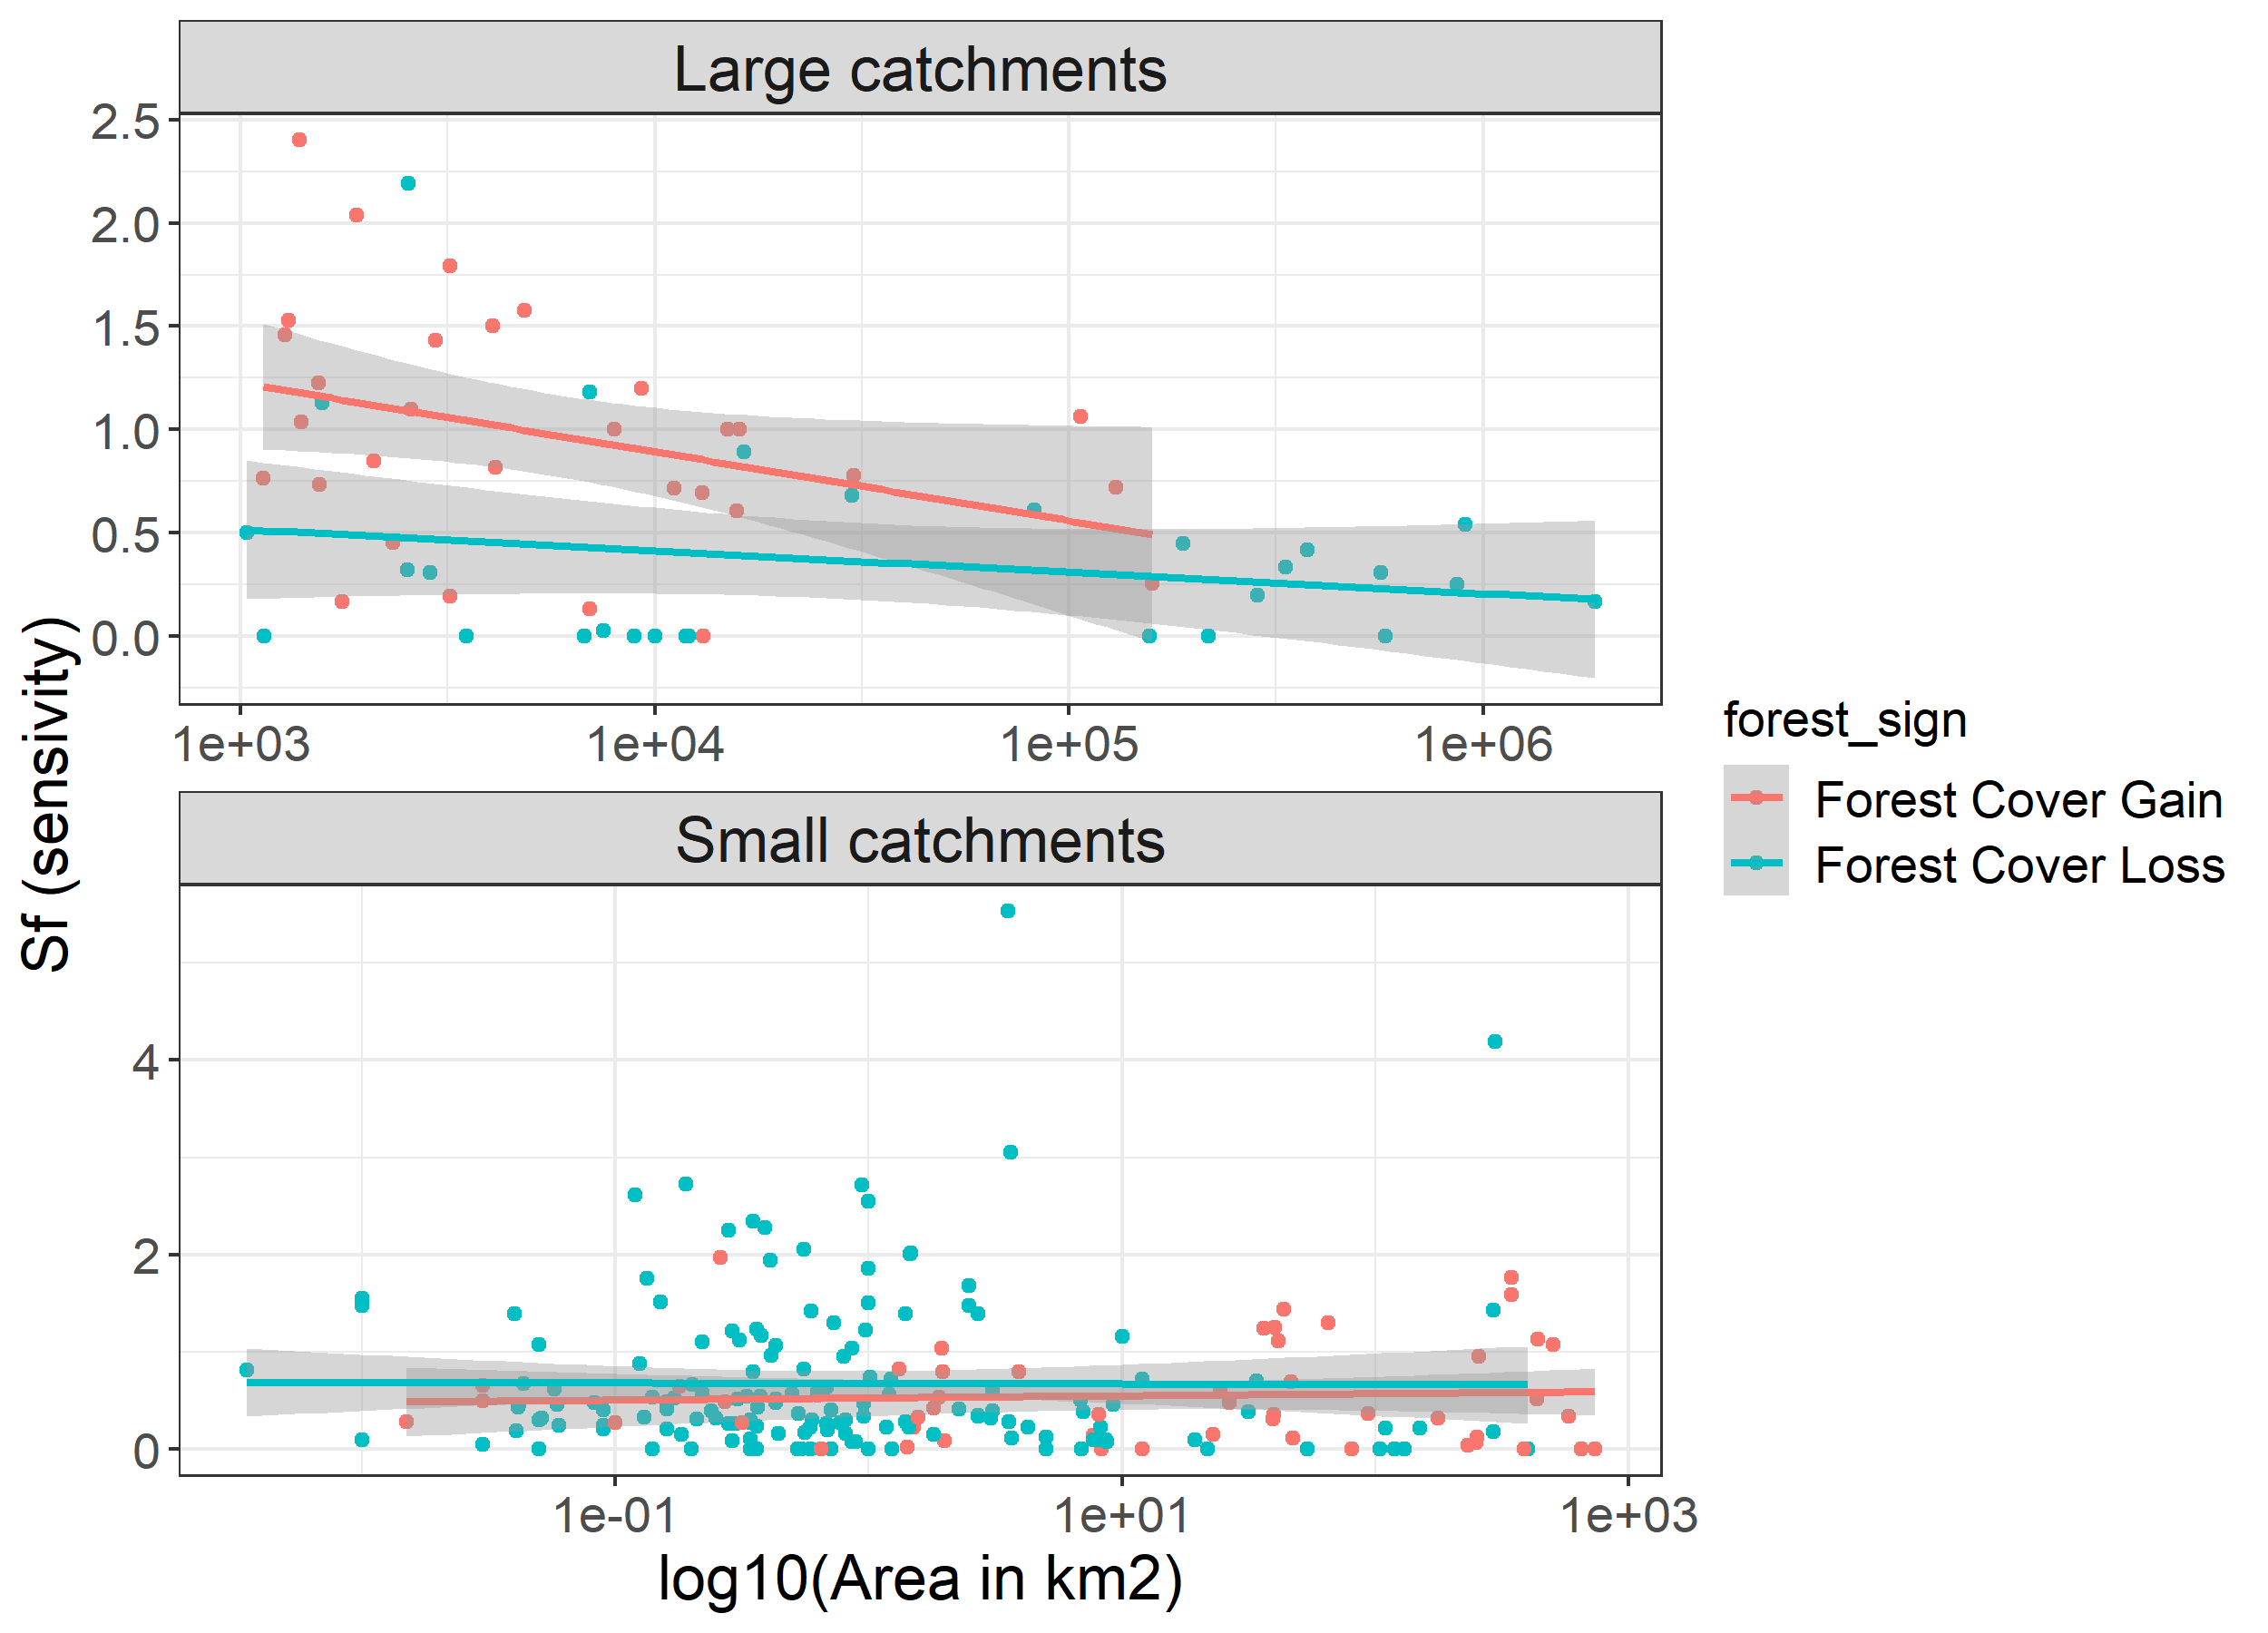
\includegraphics[width=0.9\linewidth]{Fig3Zhang} \caption{Changes in flow based on the catchments from the original data set}\label{fig:Fig3Zhang}
\end{figure}

\begin{figure}
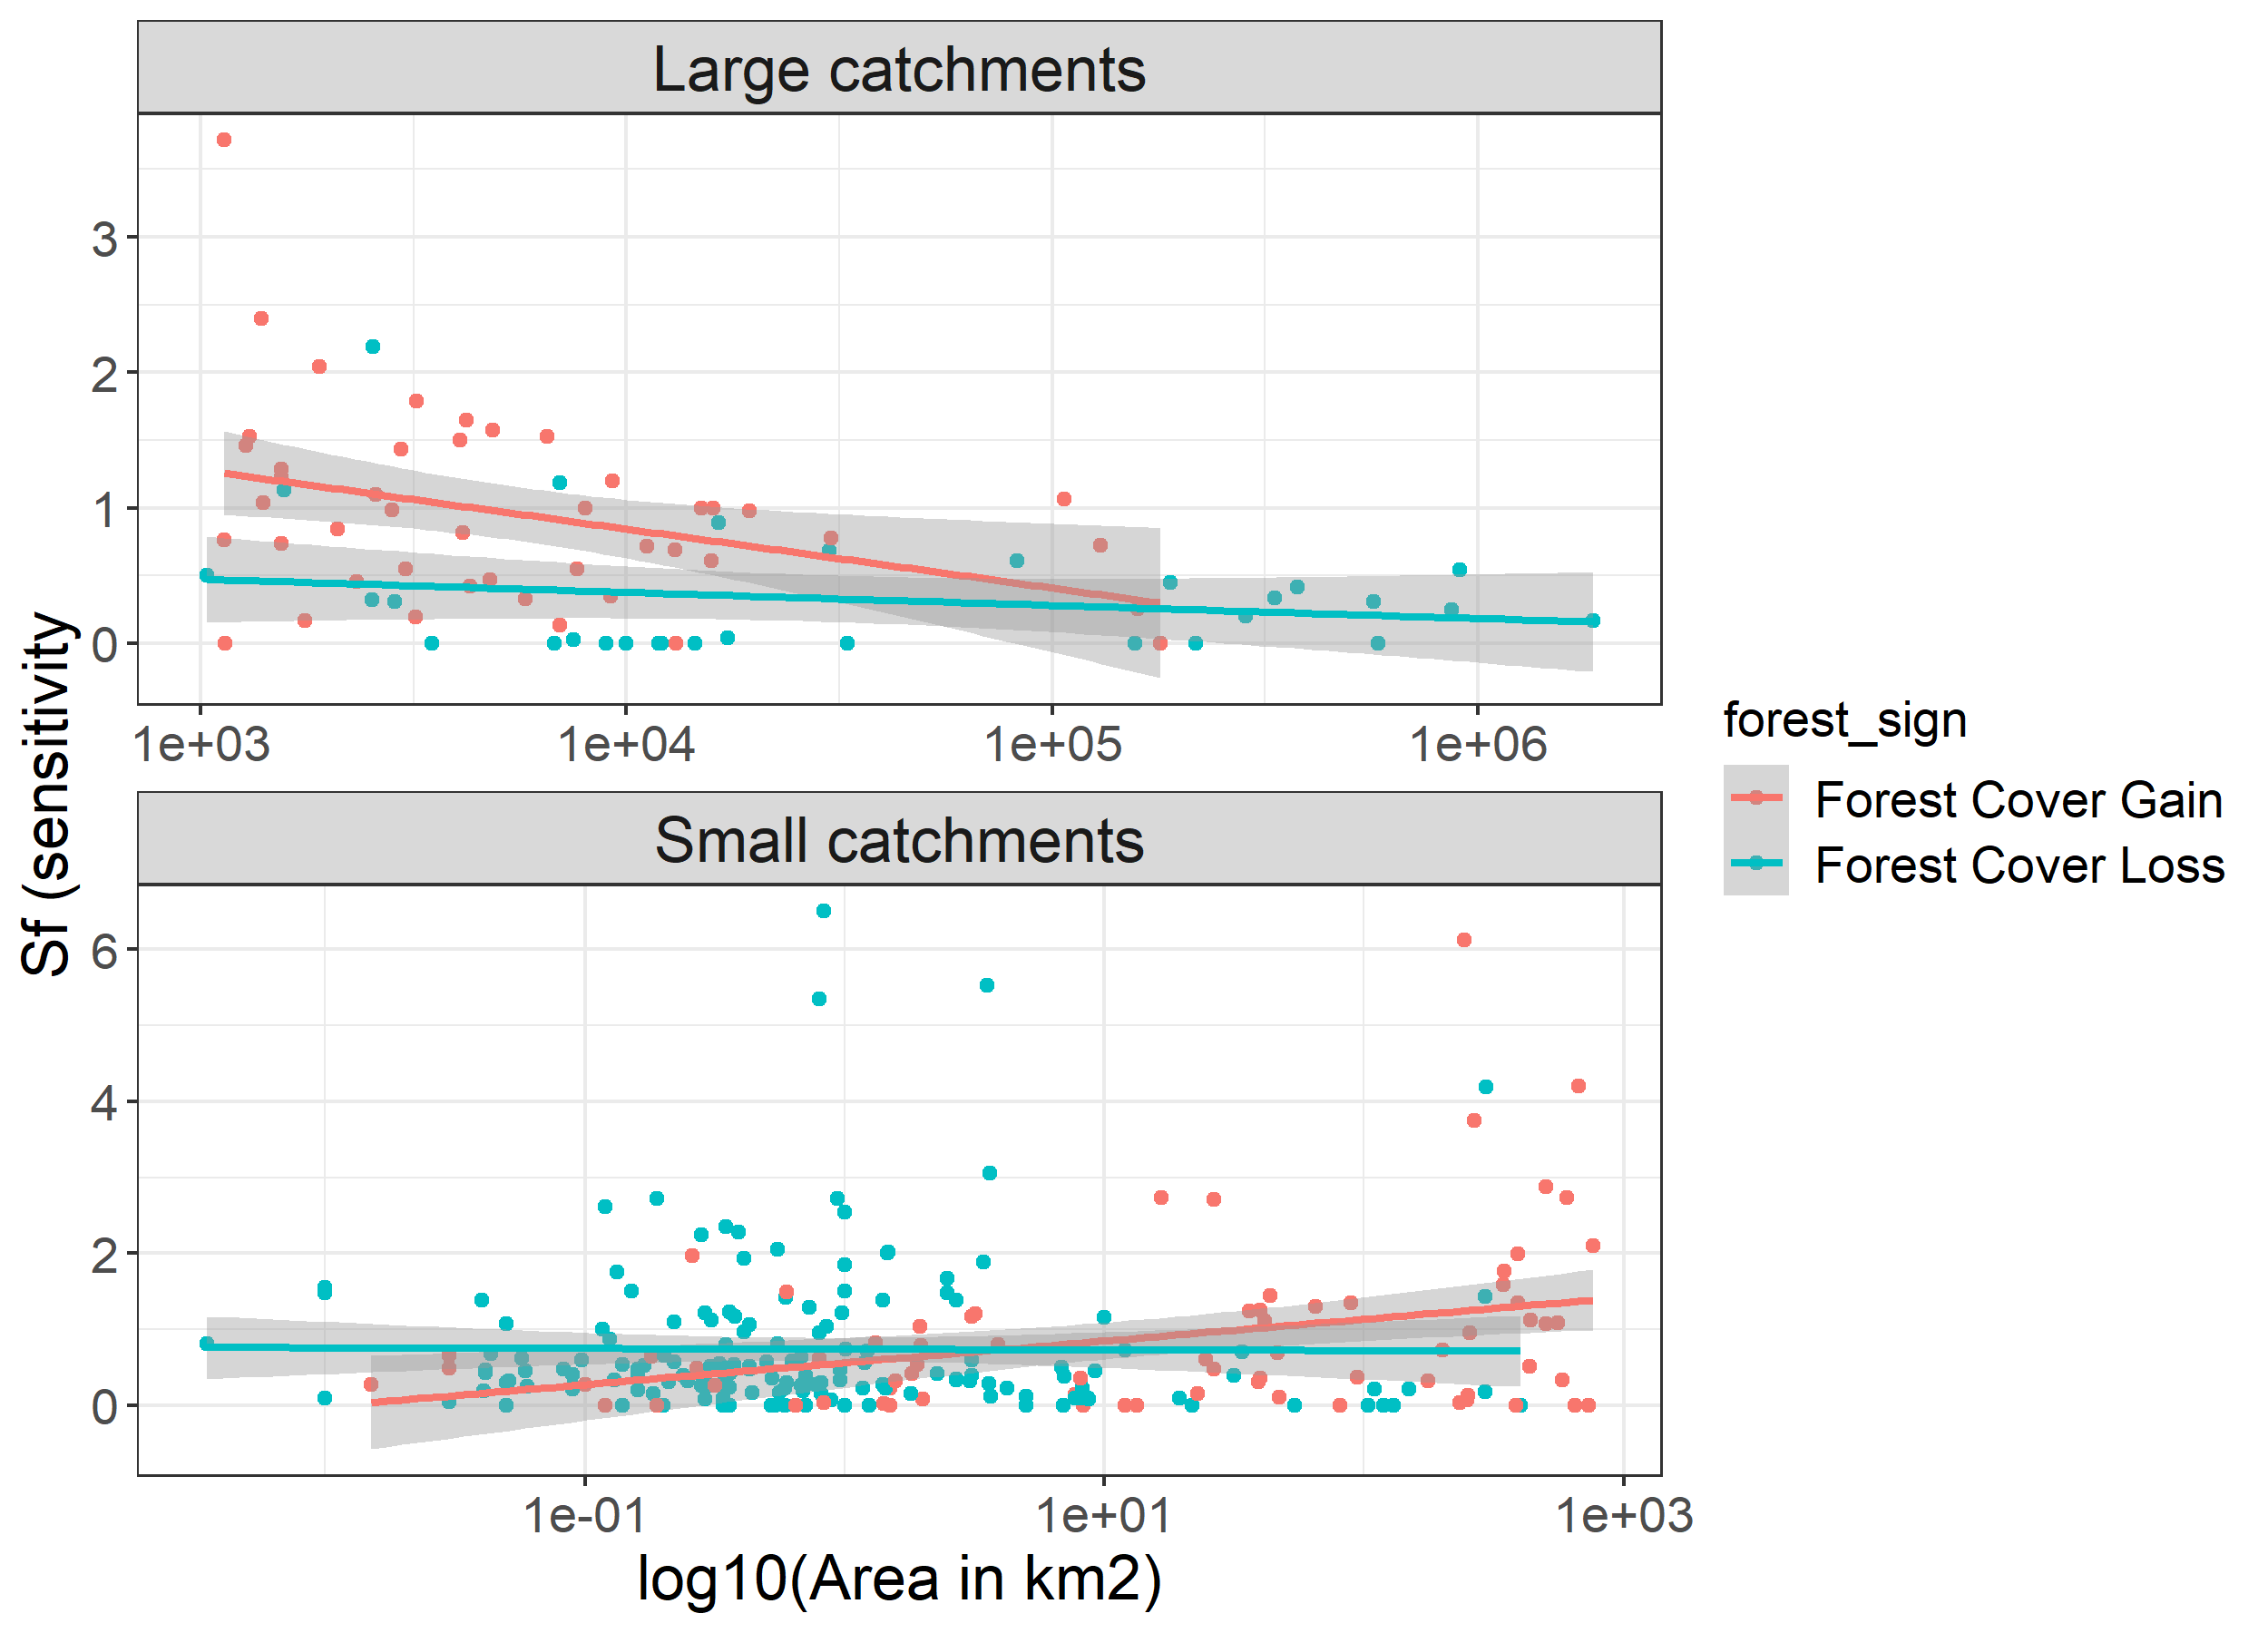
\includegraphics[width=0.9\linewidth]{Fig3Zhang_all} \caption{Changes in flow based on the catchments from the extended data set}\label{fig:Fig3Zhangnew}
\end{figure}

\hypertarget{the-sensitivity-to-forest-loss-as-a-function-of-dryness}{%
\subsection{The sensitivity to forest loss as a function of dryness}\label{the-sensitivity-to-forest-loss-as-a-function-of-dryness}}

The final analysis that we retest here is the relationship in Figure 4 in the original \citet{zhang2017} paper, which highlights the sensitivity to forest loss as a function of dryness. We are again showing just the for the small and large catchments, similar to the original paper.

Similar to earlier analyses in this document Figure \ref{fig:Fig4Zhang} show that the updated database for the original dataset results in little change in the relationships for both large and small catchments. However, when the additional new catchments are added to the database (Figure \ref{fig:Fig4Zhangnew}), the relationships clearly change. In particular, for small catchments both for forest gains and losses the relationship changes and appears stronger.

\begin{figure}
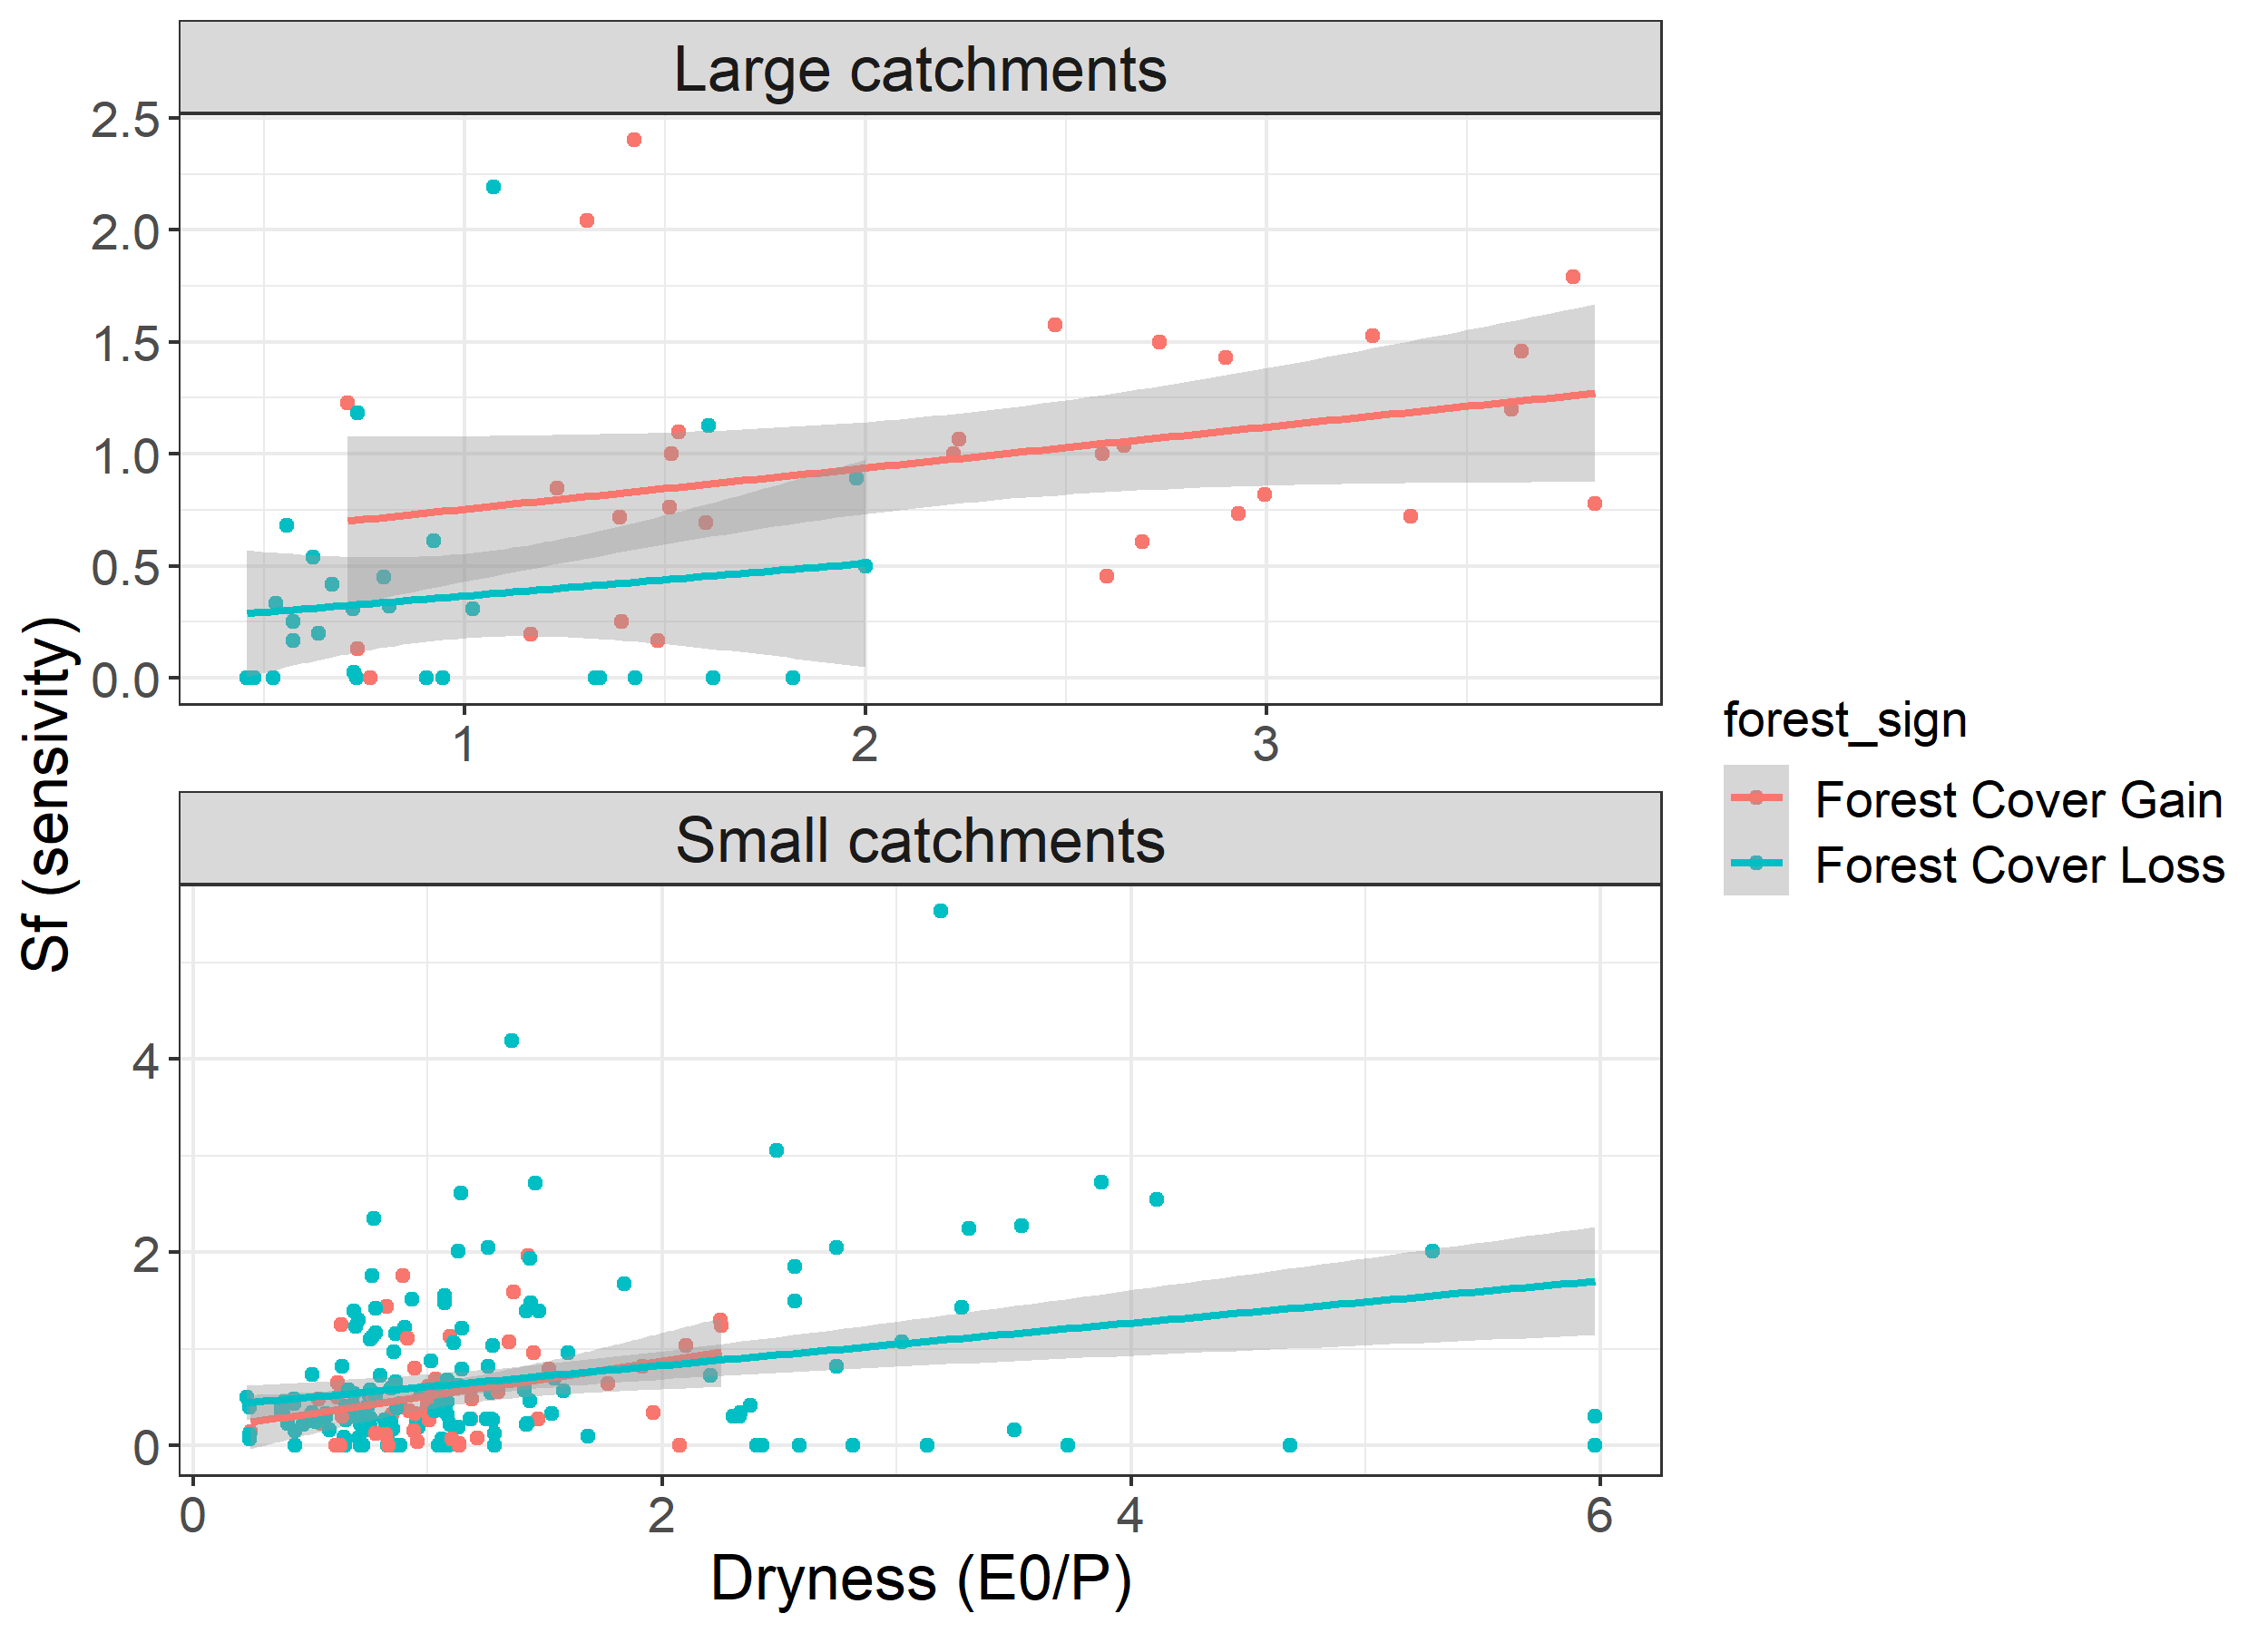
\includegraphics[width=0.9\linewidth]{Fig4Zhang} \caption{Changes in flow based on the catchments from the original data set}\label{fig:Fig4Zhang}
\end{figure}

\begin{figure}
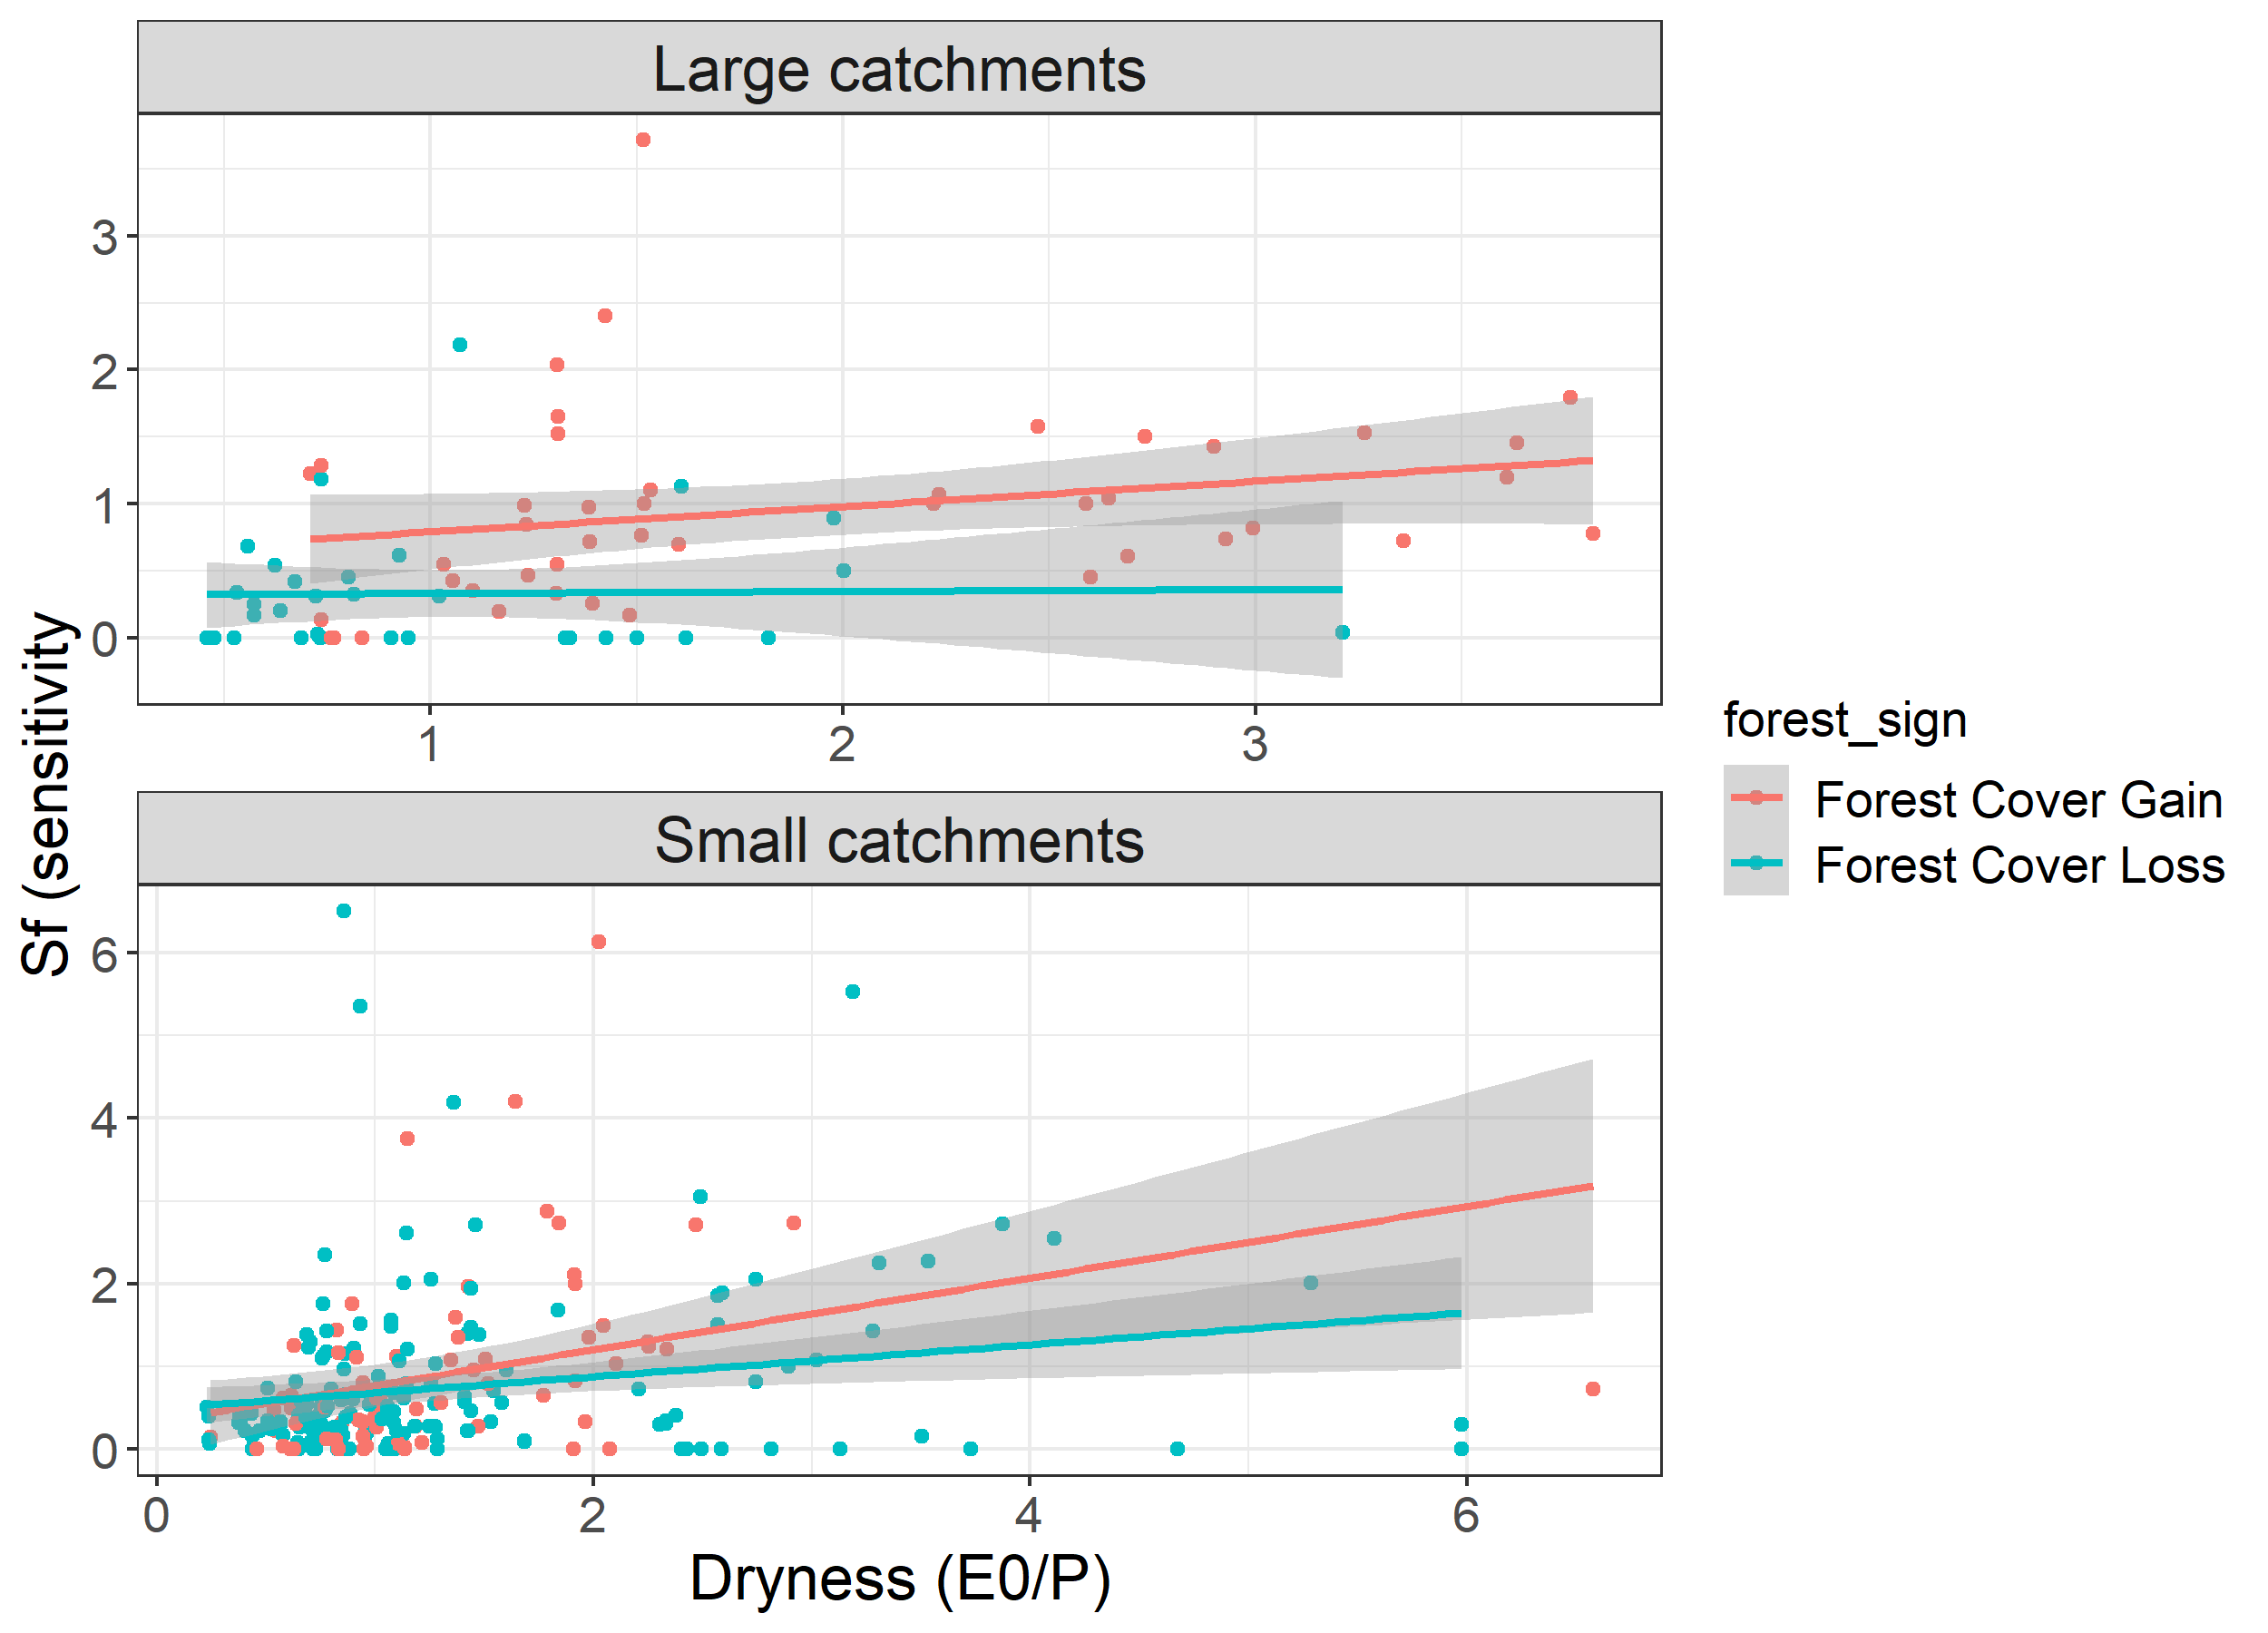
\includegraphics[width=0.9\linewidth]{Fig4Zhang_all} \caption{Changes in flow based on the catchments from the extended data set}\label{fig:Fig4Zhangnew}
\end{figure}

\bibliography{forestandwater.bib}


\end{document}
